%\section{Uma breve história do \emph{live coding}}\label{duas_ondas}

Na \autoref{sec:groove} descrevo um trabalho de \citeonline{mathews_groove_1970}, GROOVE, ainda pouco observado por \emph{live coders}. Seu paradigma composicional é diverso do MUSIC N, e o primeiro de Mathews com reflexões nos aspectos performáticos, semelhantes aos pesquisados neste trabalho.

\citeonline{mori_pietro_2015}  descreve um caso prematuro de \emph{live coding} na Itália, com o compositor Pietro Grossi (1917-2002).Divergente em algumas das propostas de Max Mathews, sacrificou a questão timbrística para trabalhar na questão performática. Esta abordagem será trabalhada na seção \autoref{sec:grossi}.

\citeonline{mclean_patterns_2009} descrevem, no final dos anos 70 e dos anos 80, atividades dos grupos \emph{The Hub} e \emph{The League of Automatic Composers} como fundamentais para o entendimento histórico do \emph{live coding}. Será explicado na seção \autoref{sec:baiasaofranscisco}

Como um breve parêntese, sugiro falar sobre a compilação JIT \cite{aycock_brief_2003}. Este é um personagem sócio-técnico fundamental para que o \emph{live coding} fosse possível. Será descrito na \autoref{sec:jit}.

Para \citeauthoronline{mclean_patterns_2009}, o \emph{live coding} não possui sua identidade cultural até a emergência da organização TOPLAP. Na \autoref{sec:laptoptoplap} proponho a revisão de um trecho da publicação ``\emph{Live Algorithm Programming and Temporary Organization for its Promotion}''.

Além deste primeiro manifesto, existe outro de grande importância, ``Show us your screens'', que define alguns cânones do \emph{live coding}. Na \autoref{sec:showusyourscreens} tratarei do caso específico.

\section{GROOVE}\label{sec:groove}

Conectando as práticas da imediaticidade, foi possível concluir que o GROOVE \cite{mathews_groove_1970,di_nunzio_genesi_2010} é um precedente mais antigo do \emph{live coding} (até que outro programa seja descoberto). Seu desenvolvimento iniciou em 1968 na \emph{Bell Labs}. Segundo o próprio Mathews, o funcionamento do sistema oferece algumas possibilidades a partir de três conceitos: criação, \emph{retroalimentação} e \emph{ciberficação}. 

O primeiro conceito foi implementado com um sistema de arquivos, onde as funções criadas no processo criativo são memorizadas, e podem ser editadas.

O segundo conceito se relaciona com o terceiro. Tange a imediatidade do fazer musical, e potencialmente, de uma necessidade de improvisação. Esta abordagem é contemporânea às técnicas de composição baseadas por \emph{retroalimentação}, como as descritas por Pauline \citeonline{oliveros_tape_1969}. Não sabemos se a primeira foi inspirada na segunda, mas o paralelo não deixa de ser significativo e importante para a concepção do que é o \emph{live coding}:

\begin{citacao}
O GROOVE provê oportunidades para uma retroalimentação imediata de observações dos efeitos das funções temporais para as entradas do computador, que compõem a função. No modo de composição do sistema GROOVE, um ser humano está em um ciclo de retroalimentação, como mostrado na figura 1 $[$\autoref{fig:groove_sistema}$]$. Assim ele é capas de modificar as funções instantâneamente como um resultado de suas observações daqueles efeitos.\cite[p.~715]{mathews_groove_1970}
\footnote{Tradução nossa de \emph{GROOVE provides opportunity for immediate feedback from observations of the effects of time functions to computer inputs which compose the function. In the compose mode of the GROOVE system, a human beign is in the feedback loop (\ldots) Thus he is able to modify the functions instanteneously as a result of his observations of their effects.}}
\end{citacao}

\begin{figure}
\begin{center}
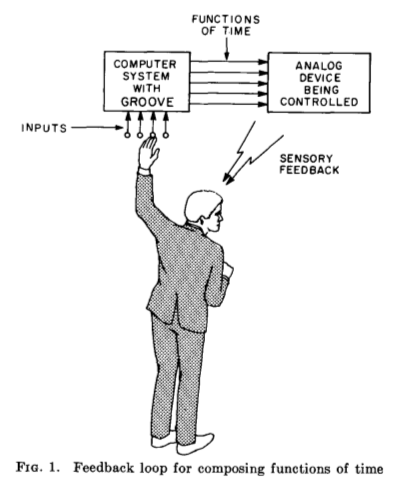
\includegraphics[scale=0.5]{./imagens/GROOVE.png}
\caption{Esquema de concepção do projeto GROOVE descrito no artigo homônimo por Max Mathews \textbf{Fonte}: \cite{mathews_groove_1970}.}
\label{fig:groove_sistema}
\end{center}
\end{figure} 

O terceiro conceito observa a existência de uma relação entre um humano e uma máquina. De certa forma, o sistema passa pr um  processo de ciberficação, considerado por Mathews como um conceito nebuloso, e chamado de \emph{engenharia humana}. Consistiu na observação de um tempo diferencial entre o que o(a) musicista cria e o que edita. De certa forma, é o conceito central que permite que os dois anteriores fossem possíveis, tange a corporificação de um regente:

\begin{citacao} 
O conceito final é mais nebuloso. Desde que o GROOVE é um sistema homem-máquina, a engenharia humana do sistema foi a mais importante. Por exemplo, nós descobrimos que o controle do programa de tempo necessita ser bastante diferente para a composição do que para a edição, e o programa foi modificado de acordo. A engenharia humana adetou toda estrutura do GROOVE de forma que pontuaremos subsequentemente. (\ldots) O intérprete de computador não deve tentar definir todo o som em tempo real. Ao invés, o computador deve ter ua partitura e o intérprete deve influenciar a forma como a partitura é tocada. Seus modoes de influência pode ser mais variados do que aqueles que um regente convencional, que pode principalmente controloar o tempo, \emph{loudness} e estilo.\cite[p.~715-716]{mathews_groove_1970}
\footnote{Tradução nossa de \emph{The final concept is more nebulous. Since GROOVE is a man-computer system, the human engeneering of the system is most important. For example, we discovered that the control of the program time needs to be quite different for composing than for editing, and the program was modiffied accordingly. Human engineering has affected the entire structure of GROOVE in ways which will be pointed out subsequently. (\ldots) The computer performer should not attempt to define the entire sound in real-time. Instead, the computer should have a score and the performer should influence the way in which the score is played. His modes of influence can be much more varied than that a conventional conductor who primarily controls tempo, loudness, and style.}.}
\end{citacao}

%O segundo ponto abordado por \citeonline{mclean_patterns_2009} no início desta subseção (1.1.1), existe uma cena de \emph{live coding} no início dos anos 2000 com as experimentações do compositor Julian Rohruber utilizando o SuperCollider\footnote{\url{http://supercollider.github.io/}, acessado em \today.}, bem como a cena musical noturna em torno do \emph{Slub}, formado por Adrian Ward, Alex McLean e Dave Griffiths \cite[p.~3]{collins_live_2003}. O \emph{SuperCollider}\footnote{\url{http://github.io.supercollider}, acessado em \today.}, inicialmente desenvolvido por James McCartney (este também um ativo praticante do \emph{live coding}), possuia apenas funcionalidades de composição algorítmica e síntese sonora em tempo-real, isto é, a demanda temporal entre o que é programado e seus resultados é consideravelmente reduzida; mas ainda assim, após uma edição, era necessário uma  reinterpretação do código\footnote{SuperCollider é uma linguagem interpretada, isto é, têm por base no código fonte linguagens compiladas. Diferentemente de linguagens como C e C++, que necessitam, dentre vários processos a compilação}. O trabalho de Rohruber, \emph{JITlib} a biblioteca \emph{Dewdrop lib} \footnote{\emph{Dewdrop} é o nome artístico de James McCartney. Para mais informações a respeito, \url{http://www.dewdrop-world.net/bio/index.html}} contribui para a conceitualização antes mesmo do \emph{Slub}. É a partir destes adventos, uma sequência de apresentações musicais e publicações de artigos que a configuração cultural do que chamarei aqui de \emph{live coding anglófono}\footnote{Inglaterra, EUA, parte inglesa do Canadá e Austrália.} começou a tomar corpo.\todo{\tiny inserir mais coisas}

\section{Pietro Grossi}\label{sec:grossi}

Embora pouco conhecido no contexto geral da música européia, o compositor Pietro Grossi foi  um dos pioneiros da \emph{Computer Music} Italiana. Diverge do \emph{paradigma} do MUSIC III e suas preocupações timbrísticas. Mas concorda, parcialmente, com a abordagem do GROOVE. Sacrificou o desenvolvimento do timbre desde o início, e para concentrar na performance, utilizou apenas uma forma de onda (pulsos). O primeiro \emph{software} desenvolvido foi o DCMP (\emph{Digital Computer Music Program}) e, segundo \cite{mori_pietro_2015}, ao usar este programa,

\begin{citacao}
(\ldots) o intéprete era capaz de produzir e reproduzir música em tempo real, digitando alguns comandos específicos e os parâmetros composicionais desejados. O som resultante vinha imediatamente depois da operação de decisão, sem qualquer atraso causado por cálculos. Haviam muitas escolhas de reprodução no programa: era possível salvar na memória do computador peças de músicas pré-existentes, para elaborar qualquermaterial sonoro no disco rígido, para administrar arquivos musicais e iniciar um processo de composição automático, baseado em algoritmos que trabalham com procedimentos ``pseudo-casuais''. Exsitia também uma abundância de escolhas para mudanças na estrutura da peça. Um dos mais importantes aspectos do trabalho de Grossi foi que todas intervenções eram instantâneas: o operado não tinha que esperar pelo computador terminar todas operações requisitadas, e depois ouvir os resultados. Cálculos de dados e reprodução sonoras eram simultâneos. Esta simultaneidade não era comum no campo da \emph{Computer Music} daquele tempo, e Grossi deliberadamente escolheu trabalhar desta forma, perdendo muito no lado da qualidade sonora. Seu desejo era poder escutar os sons resultantes imediatamente. \cite[p.~126]{mori_pietro_2015} \footnote{Tradução nossa de \emph{(\ldots) the performer was able to produce and reproduce music in real time by typing some specific commands and the desired composition's parameters. The sound result came out immediately after the operator's decision, without any delay caused by calculations. There were many reproduction choices inscribed in this software: it was possible to save on the computer memory pieces of pre-existing music, to elaborate any sound material in the hard disk, to manage the music archive and to start an automated music composition process based on algorithms that worked with “pseudo-casual” procedures. There were also plenty of choices for piece structure modifications. One of the most important aspects of Grossi’s work was that all the interventions were instantaneous: the operator had not to wait for the computer to finish all the requested operations and then hear the results. Data calculation and sound reproduction were simultaneous. This simultaneity was not common in the computer music field of that time and Grossi deliberately chose to work in this way, losing much on the sound quality’s side. His will was to listen to the sound result immediately.}}
\end{citacao}

Esta abordagem parte de uma abordagem ``preguiçosa'' (\emph{lazy}). Grossi dizia sobre si mesmo, como ``uma pessoa que está consciente de que o seu tempo é limitado e não quer perder tempo em fazer coisas inúteis ou na espera de alguma coisa quando não é necessário.''\footnote{Tradução nossa de \emph{a person who is aware that his or her time is limited and do not want to waste time in doing useless things or in waiting for something when it is not necessary.}}. Neste sentido, defendia que o desenvolvimento de novos timbres deveria esperar por melhores implementações. .

O sacrifício do timbre reflete a utilização o computador como uma paródia do piano, ou até mesmo de um violino. Grava em 1967 ``Mixed Paganini''\footnote{Disponível em \url{https://www.youtube.com/watch?v=ZQSP_wF7wSY}.}, uma execução ultra-virtuosística dos \emph{Capricci op.1} de Niccolò Paganini. Aparentemente pode soar como um pastiche musical. Porém uma escuta mais atenta permite perceber  que, a utilização de operações canônicas (inversão, aceleração e retrogradação),  executadas no computador Olivetti GE-115 \citeonline[p.~126]{mori_pietro_2015}, lembra dicotomias entre o tempo e o ritmo já discutidas por \citeonline{stockhausen_how_1957}.


\section{Baía de São Franscisco}\label{sec:baiasaofranscisco}

No final dos anos 70, na cena musical da Baía de São Fransisco, uma das atividades de John Bischoff (1949-, aluno de composição de James Tenney and Robert Ashley.) e Tim Perkis \todo{\tiny qual sua data de nascimento?} era passar horas ajustando uma rede de microcontroladores programáveis KIM-1\footnote{Disponível em \url{http://www.6502.org/trainers/buildkim/kim.htm}.}. Aquele era um momento onde os \emph{happenings} já eram manifestações artísticas consolidadas. Não demorou muito para que o público participasse da atividade:

\begin{citacao}
Na primavera de 1979, montamos uma série quinzenal regular de apresentações informais sob os auspícios da \emph{Bay Center for the Performing Arts}. Todos outros domingos à tarde passávamos algumas horas configurando nossa rede de KIMs na sala \emph{Finnish Hall}, na Berkeley, e deixávamos a rede tocando, com retoques aqui e ali, por uma ou duas horas. Os membros da audiência poderiam ir e vir como quisessem, fazer perguntas, ou simplesmente sentar e ouvir. Este foi um evento comunitário de tipos como outros compositores aparecendo, tocando ou compartilhando circuitos eletrônicos que tinham projetado e construído. Um interesse na construção de instrumentos eletrônicos de todos os tipos parecia estar "no ar". Os eventos da sala \emph{Finn Hall} foram feitos para uma cena com paisagens sonoras geradas por computador misturado com os sons de grupos de dança folclórica ensaiando no andar de cima e as reuniões ocasionais do Partido Comunista na sala de trás do edifício velho venerável. A série durou cerca de 5 meses que eu me lembre.\cite[online]{brown_indigenous_2013}\footnote{Tradução nossa de: \emph{In the spring of 1979, we set up a regular biweekly series of informal presentations under the auspices of the East Bay Center for the Performing Arts. Every other Sunday afternoon we spent a few hours setting up our network of KIMs at the Finnish Hall in Berkeley and let the network play, with tinkering here and there, for an hour or two. Audience members could come and go as they wished, ask questions, or just sit and listen. This was a community event of sorts as other composers would show up and play or share electronic circuits they had designed and built. An interest in electronic instrument building of all kinds seemed to be "in the air." The Finn Hall events made for quite a scene as computer-generated sonic landscapes mixed with the sounds of folk dancing troupes rehearsing upstairs and the occasional Communist Party meeting in the back room of the venerable old building. The series lasted about 5 months as I remember.}}
\end{citacao}

Esta experiência foi levada a cabo por Bischof, Perkis, Chris Brown (1953-), Scot Gresham-Lancaster (1954-)\footnote{Aluno de Darius Milhaud, John Chowning, Robert Ashley e Terry Riley.}, Mark Trayle (1955-)\footnote{Aluno de  Robert Ashley.} e Phil Stone\todo{\tiny ajustar informações}, que formaram nos anos 80 o grupo \emph{The Hub}, com um primeiro disco lançado em 1989 entitulado \emph{The Hub: Computer Network Music}.

Outro artista , Ron Kuivila, segundo \citeonline{mclean_patterns_2009} realiza as primeiras performances de \emph{live coding} em 1985. Um pequeno panorama de suas produções pode ajudar a entender um contexto sonoro. Em 1982 é lançada ``Going out with slow smoking'', co-produzida com Nicolas \citeonline{collins_brains_2002}\footnote{Áudio disponível em \url{http://www.nicolascollins.com/slowsmoketracks.htm}.}. Em 1985 são lançadas duas faixas em um disco peças pela \emph{TELLUS \#9 -- The Audio Casset Magazine}, ``Cannon Y for C.N.'' e ``Parodicals''. Em 1988 Kuivila grava ``Linear Predictive Zoo''\footnote{Disponível em \url{https://www.youtube.com/watch?v=DZ5pUUXqkMc}}, parte da \emph{TELLUS \#22}\footnote{Disponível em \url{http://www.discogs.com/Various-False-Phonemes/release/785540}.}.

\begin{citacao}
A primeira performance conhecida de \emph{live coding} foi em 1985, por Run Kuivila na STEIM em Amsterdã \cite{blackwell_programming_2005}. O \emph{live coding} não possui sua própria identidade cultural até o TOPLAP, a Organização Temporária para a Promoção da Programação Ao Vivo de Algoritmos, formada na \emph{Changing Grammars Workshop} em 2004 \cite{ward_live_2004}. Mesmo sendo possível pensar em fazer \emph{live coding} sem computadores, através da auto-modificação de composições baseadas em regras, não existe evidência que isto foi feito antes da invenção dos computadores. Parece que foi necessária a invenção da interpretação dinâmica de códigos para o \emph{live coding} aparecer como possível ou talvez desejável \cite[p.~1-2]{mclean_patterns_2009}\footnote{Tradução nossa de: \emph{The earliest known live coding performance was in 1985, by Ron Kuivila at STEIM in Amsterdam (Blackwell and Collins, 2005). Live coding did not get its own cultural identity until TOPLAP, the Temporary Organisation for the Promotion of Live Algorithm Programming was formed at the Changing Grammars workshop in Hamburg in 2004 (Ward et al., 2004). Although it is possible to do live coding without computers, through self-modifying rule-based composition, there is no evidence that this was done before the invention of computers. It would seem that it required the invention of dynamic code interpretation for live coding to appear possible or perhaps desirable.}}
\end{citacao}\todo{\tiny inserir mais coisas}

Embora uma breve menção de Kuivila seja realizada, é enfatizado o fato de que os construtos sócio-técnicos dos anos 80 ainda não poderiam articular o \emph{live coding} como conhecemos. Isso só foi possível com alguns desenvolvimentos técnicos e organizações de sujeitos. Como a compilação JIT \cite{aycock_brief_2003} em \emph{softwares} musicais; e a emancipação da organização TOPLAP. Antes de descrever o JIT e o TOPLAP, sugiro pensar em outras proto-histórias.

\section{Just In Time (JIT)}\label{sec:jit}

\begin{citacao}
Passageiro para o motorista: leve-me ao número 37. Eu te digo o nome da rua quando chegarmos lá.\footnote{Tradução nossa de \emph{Passenger to taxtidriver: take me to number 37. I'll give you the street name when we are there.}. Disponível em \url{http://doc.sccode.org/Overviews/JITLib.html}.}
\end{citacao}

A sentença acima é uma ``piada de um professor austríaco'' (\emph{idem, ibdem}), e descreve como este paradigma de programação em tempo-real funciona. Segundo \citeonline{aycock_brief_2003}, o primeiros programas JIT foram Genesis (com base no LISP, 1960), LC$^2$ (\emph{Language for Conversational Computing}, 1968) e APL (1970). Este último tinha duas novidades técnicas, a partir dos termos \emph{drag-along} e \emph{beating}; estes são hoje chamados de \emph{lazy evaluation} (avaliação preguiçosa). 

O \emph{SuperCollider} foi o primeiro dos \emph{softwares} descritos na introdução destre trabalho que implementou a avaliação preguiçosa.
A docuentação oferece uma descrição de como isso pode funcionar durante uma performance de \emph{live coding}:

\begin{citacao}
Para programação interativa, pode ser útil ser capaz de usar algo antes de estar ali -- isso faz o pedido de avaliação ser mais flexível e permite postergar decisões para um outro momento. Algumas preparações geralmenet tem que ser feitas (\ldots) Em outras situações este tipo de preparação não é suficiente, por exemplo se alguém quer aplicar operações matemáticas em sinais de processos sendo executados no servidor $[$do \emph{SuperCollider}$]$\footnote{Tradução nossa de \emph{For interactive programming it can be useful to be able to use something before it is there - it makes evaluation order more flexible and allows to postpone decisions to a later moment. Some preparations have to be done usually - like above, a reference has to be created. In other situations this sort of preparation is not enough, for example if one wants to apply mathematical operations on signals of running processes on the server.}. Disponível em \url{http://doc.sccode.org/Tutorials/JITLib/jitlib_basic_concepts_01.html}}
\end{citacao}

Atualmente, esta técnica têm sido largamente implementada para navegadores de internet \cite{roberts_web_2013}. Programas como Gibber\footnote{Disponível em \url{http://gibber.mat.ucsb.edu/}.} \cite{roberts_gibber:_2012} e \emph{wavepot}\footnote{Disponível em \url{https://www.wavepot.com}.} são exemplares. Durante a pesquisa, foi desenvolvido em parceria com o pesquisador Flávio Schiavonni um ambiente JIT, inspirado no GROOVE. Enquanto não foi publicado um artigo explicativo, anexamos ele no \autoref{sec:sbcm}.

\section{LAPTOP ou TOPLAP?}\label{sec:laptoptoplap}

Na \autoref{sec:perguntametodo}, \citeonline{blackwell_programming_2005} comenta a emancipação de um grupo conhecido como TOPLAP. Este acrônimo é de difícil definição. Deriva  do manifesto ``\emph{Live Algorithm Programming and Temporary Organization for its Promotion}'' \citeonline{ward_live_2004}. No \emph{Wiki} do site oficial\footnote{Disponível em \url{http://toplap.org/wiki/Main_Page}.}, a cada visita, cada letra é substituída por palavras randômicas, criando diferentes significados\footnote{Deparamo-nos, por exemplo como \emph{Transdimensional Organisation for the Pragmatics of Live Algorithm Programming}, \emph{Terrestrial Organisation for the Proliferation of Live Artistic Programming}, \emph{Temporal Organisation for the Proliferation of Live AudioVisual Programming} e outros.}.

Este manifesto expõe os ambientes de performance, bem como alguns ritos técnicos do improvisador.  Espaços de Música Eletrônica de Pista se misturam com a Música algorítmica. e Música de processos. Em outras palavras, um fenômeno onde produtores e DJs se misturam aos universitários.

\begin{citacao}
O \emph{Livecoding} permite a exploração de espaços algorítmicos abstratos como uma improvisação intelectual. Como uma atividade intelectual, pode ser colaborativa. Codificação e teorização podem ser atos sociais. Se existe um público, revelar, provocar e desafiar eles com uma matemática complexa se faz com a esperança de que sigam, ou até mesmo participem da expedição. Estas questões são, de certa forma, independentes do computador, quando a valorização e exploração de algoritmo é que importa. Outro experimento mental pode ser encarado com um DJ ao vivo codificando e escrevendo uma lista de instruções para o seu \emph{set} (realizada com o iTunes, mas aparelhos reais funcionam igualmente bem). Eles passam ao HDJ $[$ \emph{Headphone Disk Jockey} $]$ de acordo com este conjunto de instruções, mas no meio do caminho modificam a lista. A lista está em um retroprojetor para que o público possa acompanhar a tomada de decisão e tentar obter um melhor acesso ao processo de pensamento do compositor. \cite[p.~245]{ward_live_2004} \footnote{Tradução nossa de: \emph{Live coding allows the exploration of abstract algorithm spaces as an intellectual improvisation. As an intellectual activity it may be collaborative. Coding and theorising may be a social act. If there is an audience, revealing, provoking and challenging them with the bare bone mathematics can hopefully make them follow along or even take part in the expedition. These issues are in some ways independent of the computer, when it is the appreciation and exploration of algorithm that matters.   Another thought experiment can be envisaged in which a live coding DJ writes down an instruction list for their set (performed with iTunes, but real decks would do equally well). They proceed to HDJ according to this instruction set, but halfway through they modify the list. The list is on an overhead projector so the audience can follow the decision making and try to get better access to the composer’s thought process.}}
\end{citacao}\todo{\tiny inserir mais informações ou discussões}

\section{Live Algorithm Programming and Temporary Organization for its Promotion}

O manifesto ``\emph{Live Algorithm Programmin and Temporary Organization for its Promotion}'' \cite{ward_live_2004} fornece informações a respeito de comportamentos sociais e gostos musicais:

\begin{citacao}
Contudo, alguns músicos exploram suas idéias como processos de \emph{software}, muitas vezes ao ponto que o \emph{software} se torna a essência da música. Neste ponto, os músicos podem ser pensados como programadores explorando seu código manifestado como som. Isso não reduz seu papel principal como um músico, mas complementa, com a perspectiva única na composição de sua música. \textbf{Termos como ``música generativa'' e ``música de processos'' tem sido inventados e apropriados para descrever esta nova perspectiva de composição}. Muita coisa é feita das supostas propriedades da chamada ``música generativa'' que separa o compositor do resultado do seu trabalho. Brian Eno compara o fazer da música generativa com o semear de sementes que são deixadas para crescer, e sugere abrir mão do controle dos nossos processos, deixando eles ``brincarem ao vento''. \footnote{\opcit[p.~245-246]{ward_live_2004}. Tradução nossa de \emph{Indeed, some musicians explore their ideas as software processes, often to the point that a software becomes the essence of the music. At this point, the musicians may also be thought of as programmers exploring their code manifested as sound. This does not reduce their primary role as a musician, but complements it, with unique perspective on the composition of their music. Terms such as “generative music” and “processor music” have been invented and appropriated to describe this new perspective on composition. Much is made of the alleged properties of so called “generative music” that separate the composer from the resulting work. Brian Eno likens making generative music to sowing seeds that are left to grow, and suggests we give up control to our processes, leaving them to “play in the wind”.}}
\end{citacao}

Isso sumariza a prática musical do \emph{live coding} como \emph{1)} Música de Processos (\autoref{sec:alg_simples}), ou Música de algoritmos simples, \emph{2)} Música Generatva (\autoref{sec:alg_complexo}), e \emph{3)} práticas de Disk Jockey (\autoref{sec:musica_vanguarda_pista}).

\section{Música de algoritmos simples}\label{sec:alg_simples}

Segundo \citeauthoronline{wooler_framework_2005}, a música de processos é uma ``Música resultante de um conjunto de processos colocados em movimento pelo compositor, tais como  'In C' de Terry Rilley e 'It's gonna rain' de Steve Reich'' \apud[p.~1]{wooler_framework_2005}{eno_generative_1996}\footnote{Tradução nossa de \emph{Music resulting from processes set in motion by the composer “In C” by Terry Riley and “Its gonna rain” by Steve Reich}}; o que é chamado de ``procedural'' por \citeauthoronline{wooler_framework_2005}, é chamado por Joshua \citeonline{mailman_agency_2013} em seu artigo ``\emph{Agency, Determinism, Focal Time Frames and Processive Minimalist Music}'', música de processos mínimos, ou música minimalista de processos determinísticos. O autor faz menção aqui ao compositor Alvin Lucier (1931-) e sua peça \emph{Crossings} (1984). Segundo o autor,

\begin{citacao}
A longa forma de \emph{Crossings} (1984) de Alvin Lucier é especialmente clara; ela surge processivamente, neste caso de um glissando de som senoidal puro que lentamente (mais de 16 minutos) ascende de infra-sons para a ultra-sons. Um processo discreto combina com este glissando, criando uma série de processos contínuos de curto alcance. Uma orquestra dividida alterna no jogo de alturas consecutivas, em uma escala cromática ascendente ascendente que interage com o glissando. Um grupo inicia e sustenta um intervalo acima daquela do glissando de tal modo que a uma dissonância mútua cria batimentos; conforme o glissando aumenta, a velocidade do batimento diminui; quando se alcança um uníssono com os instrumentos, os batimentos momentaneamente cessam; como o glissando ascende acima da nota dos instrumentos, batimentos gradualmente aceleram. Eventualmente, o outro conjunto entra e sustenta um intervalo de um semitom acima, começando esse processo de curto alcance novamente.\cite[p.~128]{mailman_agency_2013}\footnote{Tradução nossa de \emph{The long-range form of Alvin Lucier’s Crossings (1984) is especially clear; it arises processively, in this case from a glissando of a pure sine tone that slowly (over sixteen minutes) ascends from infrasonic to ultrasonic. A discrete process combines with this glissando, creating a series of short-range continuous processes. A divided orchestra alternates in playing the consecutive pitches of a rising chromatic scale that interacts with the glissando. One ensemble initiates and sustains a pitch just higher than that of the glissando such that their mutual dissonance creates beats; as the glissando rises, the speed of the beats slows; when it reaches a unison with the instruments, the beats momentarily cease; as the glissando ascends above the pitch of the instruments, the beats gradually accelerate. Eventually, the other ensemble enters and sustains a pitch a semitone higher, starting this short-range process again.}}
\end{citacao}

Essa descrição é um breve comentário da peça, mas descreve um simples processo de ação musical, bem como relata de forma clara os resultados sonoros. É possível presumir que existe, na execução de \emph{Crossings}, um simples algoritmo que permeia toda a peça: uma alternância de um ritmo lento de dois grupos instrumentais defasados temporalmente em relação ao som emitido pelo alto-falante\footnote{Esse tipo de algoritmo pode ser facilmente implementado em uma linguagem de programação musical, como o SuperCollider (ver \autoref{crossings}).}.

Uma vez que na MP também é possível notar a influência de um algoritmo, é necessário evitar confusão com o uso original da MP, tal qual em compositores como Reich, Lucier e Riley; já o seu uso apropriado é realizado por Adrian Ward, Julian Rohruber, Frederick Olofsson, Alex McLean, Dave Griffiths, Nick Collins e Amy Alexander. Sugiro portanto comparar o fragmento do manifesto citado na página 53 com um fragmento do manifesto \emph{Music as a Gradual Process} do compositor Steve \citeonline{reich_music_1968}: 

\begin{citacao}
O que é distintivo sobre processos musicais é que eles determinam todos detalhes de nota-a-nota (som-a-som) e toda a forma simultaneamente (pense em um \emph{Round} ou um \emph{Canon}). \textbf{Eu estou interessado em processos perceptivos. Eu quero ser capaz de ouvir o processo acontecendo através da música que soa.} Para facilitar a descrição detalhada de um processo musical, a escuta  deve acontecer muito gradualmente. \cite[p.~1]{reich_music_1968}.\footnote{Tradução nossa de: \emph{The distinctive thing about musical processes is that they determine all the note-to-note (sound-to-sound) details and the over all form simultaneously. (Think of a round or infinite canon.) I am interested in perceptible processes. I want to be able to hear the  process happening throughout the sounding music. To facilitate closely detailed listening a musical process should happen extremely gradually. }}
\end{citacao}

Quanto ao manifesto de Adrian Ward, Julian Rohruber, Frederick Olofsson, Alex McLean, Dave Griffiths, Nick Collins e Amy Alexande, tenho uma primeira impressão que essa transformação gradual do som não está presente da mesma forma que em Reich, Lucier ou Rilley; vejo que o uso a reminiscência do termo ``processo'' a partir de ``procedural'' e ``processador'' se dá mais pela atividade de reprogramação em uma CGS ou CGC, mais especificamente, para fins de entretenimento. Aqui o \emph{processo} é formalizado como algoritmo, colocado na situação de constante modificação.

Já no manifesto de Reich o som não é programado, mas se prevê um comportamento musical em constante modificação a partir de uma ação mínima sobre aquilo que produz o som. Um exemplo interessante é seu \emph{Pendulum Music} (1968), onde deixa oscilar microfones posicionados acima de alto-falantes, com os cabos presos no teto; através de um único tipo de ação, restrita apenas pelas distâncias tomadas por intérpretes antes de colocar os microfones em movimento e pela comprimento do cabo preso ao teto\footnote{Seria possível incluir aqui também a resistência do ar ao movimento do objeto.}, ocorrerá um \emph{processo físico} (desaceleração das oscilações que influenciam quando o microfone passará pelo alto-falante) que desencadeará um \emph{processo perceptivo} (escuta de diferentes momentos de quando estes microfones passam pelo alto-falante até um momento estacionário). 

Tal técnica faz uso deliberado de um fenômeno conhecido como microfonia, um \emph{processo recursivo} onde os sons projetados pelo alto-falante são retro-alimentaados pelo microfone. A retroalimentação já era usada por Pauline \citeonline{oliveros_tape_1969}, como por exemplo em \emph{Beaultifoul Soup} (1967), peça para fita de dois canais, elaborada através de um circuito em retroalimentação (a compositora indica uma atividade musical econômica que ao longo do tempo causa "interessantes mudanças timbrísticas em sons sustentados" \footnote{\cfcite[p.~43]{oliveros_tape_1969} Tradução nossa de: \emph{interesting timbre changes on sustained sounds}}). Uma proposta posterior também foi realizada por Alvin Lucier (1931-) em \emph{I'm sitting in a room} (1969) quando retroalimenta seu próprio discurso em uma sala, incrementando sinais ao gravador, criando um \emph{drone}, ou um som de duração indefinida\footnote{É interessante comentar, nesse contexto, o uso deliberado de \emph{drones} no \emph{livecoding} através de uma apropriação da \emph{Drone Music}.}. Esta técnica de retroalimentação também pode ser utilizada no \emph{live coding}, por exemplo, no SuperCollider (ver \autoref{apendice_delays}).

\section{Música de algoritmos complexos}\label{sec:alg_complexo}

Esta seção discute o discurso da MG a partir de dois pontos: da perspectiva de Brian Eno, próximo à MP, e da perspectiva estrutural, pŕoxima das teorias de gramáticas generativas. A primeira será abordada na \autoref{abordagem_procedural} e a segunda na \autoref{abordagem estrutural}.
 
de Brian Eno foi mencionada por \citeonline{ward_live_2004}, farei um comentário a respeito, embora a inclusão pareça ser polisêmica a partir de um fragmento de texto de \citeonline{eno_music_1978}:

\begin{citacao}
O conceito de música projetada especificamente como pano-de-fundo ambiental foi um pioneirismo da indústria Muzak nos anos cinquenta, e tem sido conhecido genericamente como Muzak. As conotações que este termo carrega são particularmente associadas com um tipo de material que as indústria Muzak produz - melodias familiares arranjadas e orquestradas de maneira leve e derivativa. Compreensivelmente, isso leva ouvintes atentos (e compositores) a dispensar inteiramente o conceito de música ambiental como digna de atenção (\ldots) Se as empresas existentes de música enlatada se baseiam em regularizar ambientes cobrindo as idiossincrasias acústicas e atmosféricas, a Música AMbiental intenciona em melhorá-las. \textbf{Se o pano-de-fundo convencional é produzido removendo todo o sentido de dúvida e incerteza (e portanto o interesse genuíno) da música, a Música Ambiental retém essas qualidades} \cite[online]{eno_music_1978}
\footnote{\emph{The concept of music designed specifically as a background feature in the environment was pioneered by Muzak Inc. in the fifties, and has since come to be known generically by the term Muzak. The connotations that this term carries are those particularly associated with the kind of material that Muzak Inc. produces - familiar tunes arranged and orchestrated in a lightweight and derivative manner. Understandably, this has led most discerning listeners (and most composers) to dismiss entirely the concept of environmental music as an idea worthy of attention.(\ldots)Whereas the extant canned music companies proceed from the basis of regularizing environments by blanketing their acoustic and atmospheric idiosyncracies, Ambient Music is intended to enhance these. Whereas conventional background music is produced by stripping away all sense of doubt and uncertainty (and thus all genuine interest) from the music, Ambient Music retains these qualities.} Grifo nosso.}
\end{citacao} 

É interessante que neste contexto podemos fazer referência à \emph{Discreet Music} (1975) e \emph{Ambient 1: Music for Airports} (1978); tais peças fazem uso deliberado de laços de fitas que criam sistemas de atrasos (\emph{delays}). Se tais procedimento criativos não eram novos na época \footnote{Nesse sentido indicamos as peças de Steve Reich e Alvin Lucier e Pauline Oliveros já citadas.}; geralmente essas abordagens podem criar \emph{drones} que ficam variando em seu espectro.

Um exemplo interessante de \emph{live coding} com \emph{drones}, que utiliza pequenos impulsos sonoros no SuperCollider (ver \autoref{sc_drone}). Aqui o processo de escuta é contínuo, semelhante à práticas da música eletroacústica,onde algoritmos são pré-concebidos e modificados durante a performance.  Cole Ingraham utiliza um objeto que gera impulsos sonoros aperiódicos, e o mantêm como um plano sonoro que se mantêm, e vai sendo. Paralelamente, sons contínuos vai permeando este plano dos impulsos, a partir de senóides com um vibrato. É interessante notar que em alguns momentos, o \emph{live coder} deixa de programar para prestar atenção no resultado sonoro obtido, ao invés de ficar constantemente re-programando o código-fonte.

\begin{figure}
\begin{center}
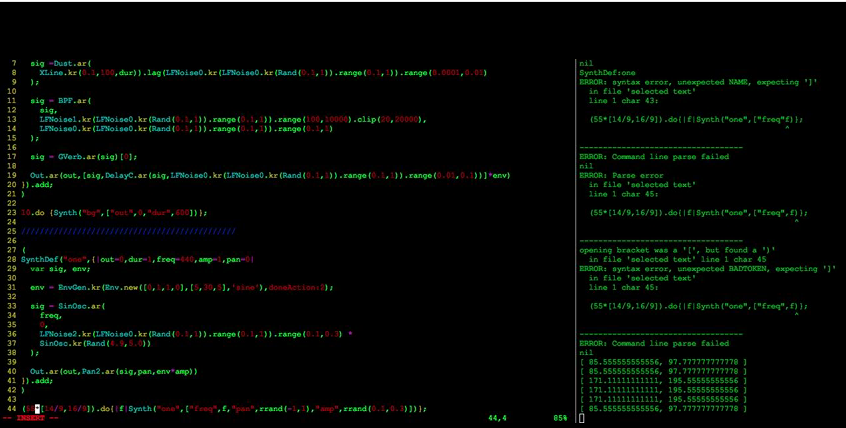
\includegraphics[scale=0.5]{./imagens/sc_drone.png}
\caption{Improviso com \emph{drones} no SuperCollider \textbf{Fonte}: \url{https://www.youtube.com/watch?v=b8j4umQ2lIE}. }
\label{sc_drone}
\end{center}
\end{figure}

\subsection{Abordagens estruturais}\label{abordagem estrutural}

Músicas realizadas a partir do \autoref{ling_estrut}, na \autoref{musica_generativa}, página 61, podem ser relacionadas com pesquisas de gramática generativa, inaugurada com o artigo ``Three Models for the description of language'' de Noam \citeonline{chomsky_three_1956}. Nesta disciplina linguística/estrutural prevalecem as implementações computacionais analíticas que possibilitam usos criativos a partir de um \textit{corpus teórico} já estabelecido\footnote{Sobre este tema sugerimos a leitura da tese "Luteria de Algoritmos Pós-Tonais" de \citeonline{soares_luteria_2015}, defendida recentemente nesta mesma instituição onde esta pesquisa está sendo realizada. Também elaborei uma peça eletroacústica nomeada \textit{Impulsos} (\url{http://soundcloud.com/opusd/musica-gerativa-9-impulsos}), onde a partir do primeiro modelo de Chomsky (cadeia Markoviana de ordem 0) e de técnicas de retroalimentação de sinais descritas por \citeonline{oliveros_tape_1969} e Alvin Lucier, elaborei uma \textit{árvore-drone} a partir de pulsos-finitos, feitos no aplicativo \emph{Wavepot} (\url{http://www.wavepot.com}), semelhantes ao som de um metrônomo.}.


Aparentemente, tais implementações podem se encaixar naquilo que Curtis \citeonline{roads_times_2001} define por \textit{Design da macroforma feita de cima para baixo}, próximo dos esquemas diretores da MA,  em contraste ao \textit{Design da macroforma feita de baixo para cima}, esta última mais próxima da MP. Sobre o termo ``de cima para baixo'' me refiro a uma abstração de alto-nível que influencia na elaboração de detalhes de uma composição; por ``de baixo para cima'' me refiro a processos elementares de uma composição, que influencia na sua macro-forma.

No entanto temos que considerar que tal dicotomia pode colocar a criatividade em campos demasiadamente rígidos, no qual outras duas abordagens podem ser tomadas para entender o aspecto \textit{linguístico}, uma negociadora entre a dicotomia e outra que elimina a dicotomia, a partir da noção de \textit{restrições}. Esta última se encaixa mais em alguns dos modelos propostos por Chomsky. Roads problematiza esta questão da seguinte maneira:

\begin{citacao}
Uma abordagem estritamente de cima-para-baixo considera a macroestrutura como um plano global pré-concebido ou um modelo cujos detalhes são preenchidos em fases posteriores da composição. Isto corresponde à noção tradicional de forma na música clássica, onde certos esquemas formais tem sido usados por compositores como moldes (Apel 1972). Muitos compositores predeterminam a macroestrutura de suas peças de acordo um um esquema mais-ou-menos formal antes de um único som ser composto. Por contraste, uma abordagem estritamente de baixo-para-cima concebe a forma como resultado de um processo de desenvolvimento interno provocado por interações nos níveis mais baixos da estrutura (\ldots) Para alguns, composição envolve uma mediação entre as abordagens de cima-para-baixo e de baixo-para-cima, entre uma concepção abstrata de alto-nível e os materiais concretos sendo desenvolvidos nos níveis mais baixos da estrutura. Isso implica uma negociação entre o desejo de ordenar a macroestrutura e imperativos que emergem da fonte material (\ldots) Ultimamente, a dicotomia entre forma e processo é uma ilusão, uma falha da linguagem para cegar dois aspectos do mesmo conceito em uma unidade. Nas ciências da computação, o conceito de \textit{restrição} elimina esta dicotomia (Sussman and Steele 1981). Uma forma é construída de acordo com um conjunto de relações. Um conjunto de relações implica um processo de avaliação que resulta em uma forma.  \cite[p.~12-14]{roads_times_2001}
\footnote{Tradução nossa de:\textit{A strict top-down approach considers macrostructure as a preconceived global plan or template whose details are filled in by lates stages of composition. This corresponds to the traditional notion of form in classical music, wherein certain formal schemes have been used by composers as molds (Apel 1972). (\ldots) Many composers predetermine the macrostructure of their pieces according to a more-or-less formal scheme before a single sound is composed. By contrast, a strict bottom-up approach conceives of form as the result of a process of internal development provoked by interactions on lower levels of musical structure (\ldots) For some, composition involves a mediation between the top-down and bottom-up approaches, between an abstract high-level conception and the concrete materials beign developed on lower levels of musical structure. This implies negotiation between a desire for ordely macrostructure and imperatves that emerge from source material (\ldots) Ultimately, the dichotomy between form and process is an illusion, a failure of language to bind two aspects of the same concept into a unit. In computer science, the concept of constraints does away with this dichotomy (Sussman and Steele 1981). A form is constructed according to a set of relationships. A set of relationships implies a process of evaluation that results in form}}
\end{citacao}

Restrições são pequenas regras, que se assemelham a gramáticas; tais gramáticas, podem depender métodos e técnicas de composição que restringem possibilidades criativas, afim de gerar novas restrições e possibilidades. Esta categoria de composições dependem de um corpo teórico bem estabelecido, procedendo primeiramente através da análise; tais análises podem partir como a Teoria de níveis estruturais de Heinrich Schenker, da Teoria Generativa da Música Tonal de Lerdhal e Jackendoff  (GTTM) e a Teoria de Implicação-Realização de Eugene Narmour, para depois agir criativamente; tais análises indicariam comportamentos direcionais, melódicos, harmônicos e rítmicos de uma composição, colocando este aspecto como relativo a algumas produções da música tonal européia \footnote{\cfcite[p.~29--43]{rowe_machine_1991}}.

No \emph{live coding}, essa abordagem pode ser realizada com o \emph{Tidal} de \citeonline{mclean_tidal_2010}\footnote{``\emph{Tidal} é uma lingagem de padrões embebida na linguagem de programação Haskell, consistindo de representações de padrões, uma biblioteca de geradores de padrões'' \cite[p.~2]{mclean_tidal_2010}. Tradução nossa de \emph{Tidal is a pattern language embedded in the Haskell programming language, consisting of pattern representation,a library of pattern generators and combinators, an event scheduler and programmer’s live coding interface.}}., como na \autoref{fig:lc_tidal}. % observamos o seguinte uso: de $0'05''$ a $0'22''$, Mark Derricutt define um pulso básico como um bumbo; de $0'22''$ a $0'38''$, define um outro som, semelhante ao bumbo, mas com mais graves no ataque que o primeiro, em contra-tempo com o pulso básico (o que por si só caracteriza uma performance de \emph{algorave}). De $0'38''$ a $1'05''$, define quatro semicolcheias. De $1'05''$ a $1'16''$, executa uma permutação com esses materiais. De $1'16''$ a $1'26''$ , o ritmo se torna mais complexo, mas com base no bumbo inicial. De $1'26''$ a $1'51''$, é alterado o pulso original, tornando o ritmo anterior mais lento. De $1'51''$ a $2'02''$, entra um ``baixo''', em contra-tempo com o 3$^o$ tempo da célula rítmica; do ponto de vista de gênero musical, o nome do som utilizado para o baixo é o ``gabba'', um tipo de ``Hardcore dance'' surgido em 1993 na Holanda, e também conhecido como \emph{Rotterdam techno}\footnote{Conferir \url{http://corehistory.blogspot.com.br/2009/12/gabber.html}.}. A partir de $2'02''$ a $3'25''$ o \emph{live coder} improvisa com um material chamado \emph{industrial} (outro possível gênero musical para a performance), manipulando-o através de DSPs que se assemelham a filtros de vogais (aeiou). De $3'25''$ a $4'25''$ um novo material melódico, sincopado, é incluído (\emph{arpy}, provavelmente semelhante aos sintetizadores ARP); é interessante notar que as alturas dessa melodia são permutadas. De $4'25''$ a $4'57''$, essa melodia é panoramizada, isto é, uma onda senoidal controla a posição estereofônica da melodia, como se ela girasse em torno da cabeça do ouvinte. Em $4'57''$ a $5'22''$  é aplicado um \emph{delay} nesta melodia, isto é, as notas serão repetidas, criando uma espécie de \emph{canon}. Em $5'22''$ o mesmo procedimento de panoramização é aplicado ao baixo. Em $5'58''$ a $6'26''$, a melodia em \emph{canon} é alterada para tocar com pausas entre algumas notas, sem o \emph{delay} que gerava o \emph{canon} que se mantém até o final em $7'04''$

\begin{figure}
\begin{center}
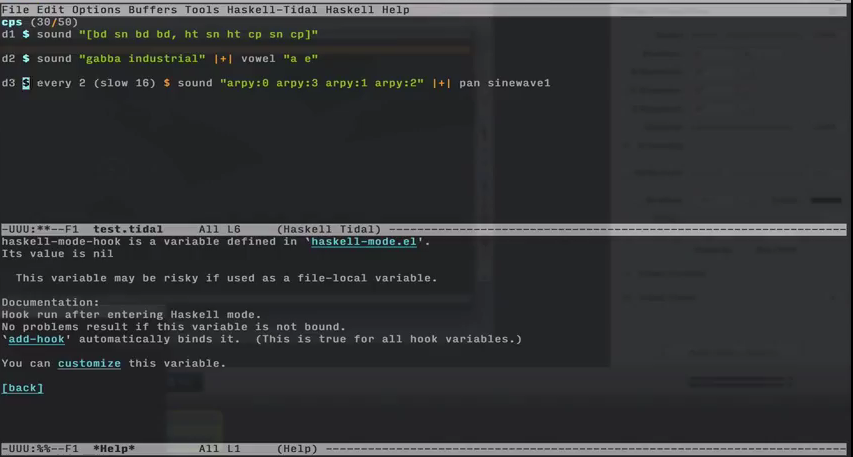
\includegraphics[scale=0.5]{./imagens/tidal.png}
\caption{\emph{Live coding} com Tidal \textbf{Fonte}: \url{https://www.youtube.com/watch?v=ZQqg9Ghxruo}.}
\label{fig:lc_tidal}
\end{center}
\end{figure}

\section{Prática DJ}\label{sec:musica_vanguarda_pista}

Somado a todos esses elementos, existe a imagem já descrita de um DJ que se utiliza destas técnicas e estéticas para controlar seu \emph{set} (embora seja possível assumir que esta personagem pode utilizar outros dispositivos, como sintetizadores e baterias eletrônicas, todos eles presentes em um computador) e promover uma música na qual a dança é elemento central. É importante deixar claro que uma cultura DJ possui suas peculiaridades dependentes de contexto social: por exemplo, um dj europeu/norte-americano está em uma configuração social diversa do dj latino-americano e africano. Se até o momento temos discutido práticas musicais, na sua maioria, a partir de pessoas que falam o inglês como sua primeira língua, é natural supor que esta cultura DJ que falamos no \emph{livecoding} faz parte de uma cultura anglófona.

Esse fenômeno de apropriação das MA, MG, MP e DJ, na cultura musical dos países rotulados como desenvolvidos, pode ser entendido a partir daquilo que Fernando  \citeonline{iazzetta_musica_2009} chamou de "sinergia de produções, que em sua diversidade compartilham dos mesmos elementos sociais e culturais" \cite[p.~152]{iazzetta_musica_2009}. Mais especificamente, trata-se de um fenômeno em sentido mais amplo das produções musicais usando o computador; mas buscarei encarar a questão no \emph{livecoding} da mesma maneira, como uma sinergia entre boates, casas noturnas e ambientes informais com ambientes de produção de conhecimento (universidades, escolas de música, faculdades de engenharia).

Primeiro é necessário esclarecer se a apropriação foi intencional ou não.  O discurso do manifesto de \citeonline{ward_live_2004} indica uma consciência parcial dos autores a respeito desta sinergia. No entanto é discutível se esse cruzamento de gêneros é mais um reflexo das transformações sociais e culturais que o computador trouxe consigo do que algo intencional: o uso deliberado de muitas ferramentas de um estúdio portátil, a expansão de possibilidades de produção musical através das redes de computadores, a troca de informações a respeito do uso de novos \emph{softwares} entre músicos acadêmicos e não-acadêmicos , trouxe à tona diferentes comunidades daquela ou outra tecnologia. De forma semelhante, no \emph{livecoding}, as novas possibilidades tecnológicas em contato com modos de fazer música já estabelecidos possiblitaram a emancipação de novas práticas, o que por sua vez, capacitou o cruzamento de estéticas (tudo isso, no entanto, visto apenas pela ótica das culturas de pessoas que falam o inglês como primeira língua).

Poderia ser questionado se o intercruzamento de gêneros musicais no \emph{livecoding} depende dos \emph{softwares}.  \citeauthoronline{iazzetta_musica_2009} responderia não, mas que dependem de uma articulação entre produções musicais e seus compositores, que carregam diferentes formações teóricas. Esse problema é colocada da seguinte forma:


Embora seja possível considerar uma "comunidade Max/MSP", ela está dentro de uma população contendo as comunidades "SuperCollider", "PureData", "ChucK", indicando apenas alguns. 

Dentro dessa população, surgem as pequenas comunidades de \emph{softwares} de \emph{live coding}, pela utilização e invenção de mini-linguagens pouco usadas, se comparadas com as do parágrafo acima. No contexto anglófono, essas pequenas comunidades apropriam um termo, segundo \citeonline{collins_algorave:_2014}, \emph{algorave}. 

Algorave é  um tipo de música eletronica de pista, que se utiliza de algoritmos, processos, e teorias generativas;  não se configura como uma música de pista normal, em seu processo de criação, mas reproduz alguns regimes de escuta, como \emph{dance}, \emph{drum'n'bass}, \emph{cyberpunk}, etc. Nesse processo de criação, é comum utilizar alguns \emph{softwares} já comentados, como o \emph{iXiLang} e o \emph{Tidal}, o que leva a crer na emancipação de ``comunidades iXiLang'' e ``comunidades Tidal''.

No entanto, \emph{algorave} é um termo anterior ao advento do \emph{live coding} e ao uso dos \emph{softwares} supracitados:

\begin{citacao}
\emph{Algorave} não é sustentado exclusivamente por \emph{live coders}, mas estes têm mantido uma forte presença em todos os eventos até agora. É assim talvez, porque a tradição do \emph{live coding} de projetar telas motiva todo o esforço; onde algoritmos não estão visíveis por períodos de tempo durante uma algorave, se corre o risco das coisas parecerem muito como um evento de música eletrônica padrão. \cite[p.~356]{collins_algorave:_2014} \footnote{Tradução nossa de \emph{Algorave is not exclusively a preserve of live coders, but they have maintained a strong presence at every event thus far. This is perhaps because the live coding tradition of projecting screens help motivates the whole endeavour; where algorithms are not made visible for periods during an algorave, we run the risk of things feeling much like a standard electronic music event.}}
\end{citacao}


\citeauthoronline{collins_algorave:_2014} apresenta dados a respeito da história da \emph{algorave}: em 1992 uma performance entitulada \emph{Cybernetic Composer} de Charles Ames; passando pelo \emph{Aphex Twin} (Richard David James), que  reinvindica em 1997 o termo (interessante do ponto de vista de gênero musical) \emph{live club algorithm}; em 2000 o \emph{Slub}, citado no inicio deste capitulo (na época Adrian Ward, Alex McLean), realizam performances, autodenominadas \emph{generative techno}, com abordagem \emph{gabba}; é interessante aqui o uso do termo \emph{club live coding}. Em 2001 é identificado a utilização de redes neurais para composição de padrões semelhantes ao \emph{drum'n'bass}. Em 2004 é fundado o TOPLAP, organização internacional  de \emph{live coding}, em uma casa noturna de Hamburgo. \footnote{\loccit{collins_algorave:_2014}.}

 

\section{\emph{Show us your screens}}\label{sec:showusyourscreens}

Além das performances inaugurais nos festivais Europeus, e do manifesto ``Live Algorithm Programming and Temporary Organization for its Promotion'', um texto possui uma importância fundamental para \emph{live coding}. Premissas de comportamentos e técnicas são delineadas no texto ``\emph{Show Us Your Screens}''\cite[p.~22; online]{griffiths_fluxus:_2008,mccallum_show_2011}:\todo{\tiny Aqui as correções ainda não foram aplicadas, apenas sessões foram ajustadas, suas ordens}

\begin{citacao}
Exigimos:

• Acesso à mente do intérprete, para todo o instrumento humano.

• Obscurantismo é perigoso. Mostre-nos suas telas.

• Programas são instrumentos que podem modificar eles mesmos.

• O programa será transcendido - Língua Artificial é o caminho.

• O código deve ser visto assim como ouvido, códigos subjacentes visualizados bem como seu resultado visual.

• Codificação ao vivo não é sobre ferramentas. Algoritmos são pensamentos. Motosserras são ferramentas. É por isso que às vezes algoritmos são mais difíceis de perceber do que motosserras.

Reconhecemos contínuos de interação e profundidade, mas preferimos:

• Introspecção dos algoritmos.

• A externalização hábil de algoritmo como exibição expressiva/impressiva de destreza mental.

• Sem \emph{backup} (minidisc, DVD, safety net computer).

Nós reconhecemos que:

• Não é necessário para uma audiência leiga compreender o código para apreciar, tal como não é necessário saber como tocar guitarra para apreciar uma performance de guitarra.

• Codificação ao vivo pode ser acompanhada por uma impressionante exibição de destreza manual e a glorificação da interface de digitação.

• Performance envolve contínuos de interação, cobrindo talvez o âmbito dos controles, no que diz respeito ao parâmetro espaço da obra de arte, ou conteúdo gestual, particularmente direcionado para o detalhe expressivo. Enquanto desvios na tradicional taxa de reflexos táteis da expressividade, na música instrumental, não são aproximadas no código, por que repetir o passado? Sem dúvida, a escrita de código e expressão do pensamento irá desenvolver suas próprias nuances e costumes.
\footnote{Tradução nossa de:\emph{We demand: \begin{inparaenum}[•]
\item Give us access to the performer's mind, to the whole human instrument.
\item Obscurantism is dangerous. Show us your screens.
\item Programs are instruments that can change themselves.
\item The program is to be transcended - Artificial language is the way.
\item Code should be seen as well as heard, underlying algorithms viewed as well as their visual outcome.
\item Live coding is not about tools. Algorithms are thoughts. Chainsaws are tools. That's why algorithms are
sometimes harder to notice than chainsaws.
\end{inparaenum}. We recognise continuums of interaction and profundity, but prefer:  \begin{inparaenum}[•]
\item Insight into algorithms
\item The skillful extemporisation of algorithm as an expressive/impressive display of mental dexterity
\item No backup (minidisc, DVD, safety net computer)
\end{inparaenum}. We acknowledge that: \begin{inparaenum}[•]
\item It is not necessary for a lay audience to understand the code to appreciate it, much as it is not necessary
to know how to play guitar in order to appreciate watching a guitar performance.
\item Live coding may be accompanied by an impressive display of manual dexterity and the glorification of the
typing interface.
\item Performance involves continuums of interaction, covering perhaps the scope of controls with respect to
the parameter space of the artwork, or gestural content, particularly directness of expressive detail. Whilst
the traditional haptic rate timing deviations of expressivity in instrumental music are not approximated in
code, why repeat the past? No doubt the writing of code and expression of thought will develop its own
nuances and customs.
\end{inparaenum}}}
\end{citacao}

``Dar acesso à mente do intérprete'' e ``obscurantismo é perigoso'' descrevem um meio de evitar qualquer código mal intencionado; isto é uma hipótese: \begin{inparaenum}[\itshape i)\upshape]
\item programas de \emph{live coding} geralmente são programas em fase de desenvolvimento;
\item programas em desenvolvimento possuem, inevitavelmente, \emph{bugs}\footnote{Segundo James S. Huggins, historicamente ``O termo \emph{bug} é usado de forma limitada para designar qualquer falha ou problema em conexões ou no trabalho com aparatos elétricos'' Tradução nossa de \emph{The term "bug" is used to a limited extent to designate any fault or trouble in the connections or working of electric apparatus.} (ver \url{http://www.jamesshuggins.com/h/tek1/first_computer_bug.htm}). Nesse sentido, um \emph{bug} em um programa é uma falha de operação, geralmente causada por algum erro de lógica, por parte do programador.}
\item \emph{bugs} podem ser explorados e levar à corrupção do sistema.
\end{inparaenum} Se esta hipótese estiver correta, justificaria a atitude de exposição da \emph{imagem-texto}. No entanto não encontrei algum estudo crítico descrevendo se isso é verdade a partir do ponto de vista do público, isto é, será que o público pode estar realmente interessado na exposição da \emph{imagem-texto}? Será que essa exposição não pode ser perigosa para o processo artístico e para a experiência do público? Embora sejam questões que fogem do escopo do trabalho, são importantes, necessitando verificar algumas performances para averiguar.

``Programas são instrumentos'' e ``O programa será transcendido - Língua Artificial é o caminho'', são frases que fazem menção direta à experiência de usuário (\emph{live coder}), isto é, um sistema que é programável de maneira facilitada. A seguinte hipótese pode ser feita: quanto mais simplificada a linguagem de programação, mais expressão visual ou musical um espetáculo poderá ter (o que pode não ser verdade, e sim que a expressão musical estaria no nível sensível). Por ``Língua Artifical'' entendo que o \emph{live coder} pode criar \emph{mini-linguagens} ou Linguagens de Domínio Específico (DSL)\footnote{Sobre esse tema recomendo o texto ``Minilanguages, finding a notation that sings'' de \citeonline{raymond_minilanguages_2003}: ``Historicamente, linguagens de dominio especifico sao do tipo que sao chamadas de 'pequenas linguagens' ou 'minilinguagens' no mundo do Unix, porque os primeiros exemplos eram pequenos e de pouca complexidade, em relaçao às linguagens de propósito geral (\ldots) Nós manteremos o termo tradicional 'minilinguagem'para engatizar que no decorrer do curso é geralmente utilizado para projetar e mantê-las o menor e simples possível'' \cite[$3^o$ parágrafo]{raymond_minilanguages_2003}. Tradução nossa de \emph{Historically, domain-specific languages of this kind have been called ‘little languages’ or ‘minilanguages’ in the Unix world, because early examples were small and low in complexity relative to general-purpose languages (\ldots) We'll keep the traditional term ‘minilanguage’ to emphasize that the wise course is usually to keep these designs as small and simple as possible.}} que possibilitam criar programas para criar um espetáculo audiovisual ou musical. Segundo \citeonline{collins_algorave:_2014}, tais DSLs estariam no formato de ``mini-linguagens'' bem desenvolvidas para a tarefa específica de codificar música ao vivo, operando técnicas composicionais como a transformação de um padrão musical (como por exemplo, técnicas barrocas como inversão e retrogradação ou técnicas aleatórias, como emabaralhamento de um conjunto de eventos sonoros), facilitando a espontaneidade no processo criativo:

\begin{citacao}
Existe um número crescente de sistemas de \emph{livecoding} com ``mini-linguagens'' amigáveis, que facilitam o \emph{loop} e contruções de camadas centrais típicas para dançar música. \emph{Ixilang} é um exemplo primário, e possui um editor de código estruturado que, enquanto baseado em texto, suporta correspondências visuais. \emph{Tidals} é outro, e, embora com foco na rapidez de utilização ao invés da facilidade de aprendizagem, está começando a ter mais ampla aceitação. Ambos \emph{ixilang} e \emph{Tidal} promovem padrões em termos de funções transformadoras como embaralhamento, inversão e extrapolação de formas diferentes.  \cite[p~.357]{collins_algorave:_2014}\footnote{Tradução nossa de: \emph{There are increasingly user friendly “mini-language” livecoding systems which facilitate loop and layer-centric con-structions typical to dance music. ixilang is a primary example, and features a structured code editor which while text-based, supports visual correspondences. Tidal is another, and although its focus is on speed of use rather than ease of learning, is beginning to see wider take-up. Both ixilang and Tidal promote pattern in terms of transformative functions as scrambling, reversal and extrapolation in different ways}.}
\end{citacao}


``O código deve ser visto assim como ouvido'' entraria em um problema próprio de programas de pesquisa em notação musical, sendo que o processo de correlação entre o que está escrito e o que está sendo ouvido leva um tempo ou pode mesmo nem existir. Mesmo com o convite expressado pelo manifesto ``\emph{Live Algorithm Programming and Temporary Organization for its Promotion}'' no início do capítulo, a questão não está nem no uso do computador nem em alguma abordagem musical, e conforme a performance avança, a imagem-texto vai se tornando tão poluída que poderia causar um desinteresse.

\begin{citacao}
Codificação e teorização podem ser atos sociais. Se existe um público, revelar, provocar e desafiar eles com uma matemática complexa se faz com a esperança de que sigam, ou até mesmo participem da expedição. Estas questões são, de certa forma, independentes do computador, quando a valorização e exploração de algoritmo é que importa.\cite[p.~204]{ward_live_2004}
\end{citacao}

``Algoritmos são pensamentos. Motosserras são ferramentas.'', ``Introspecção dos algoritmos.'' e ``A externalização hábil de algoritmo'' descrevem uma atividade constante de formalizações lógicas, do processo febril de explorar uma complexidade própria do que se criou, de ficar digitando sem parar um teclado de computador. Alguns colegas e amigos não programadores, músicos e não músicos, utilizam a expressão ``gostar de apertar botão'' para se referir à caricatura do programador em um espaço reservado, no qual controla dispositivos diversos.

``Sem \emph{backup}'' indica o comportamento do \emph{live coder} após uma improvisação, que não memoriza em discos rígidos, cd's ou \emph{pendrives} o documento criado (isto é, o código textual, em alguma extensão apropriada para a linguagem utilizada, por exemplo, \emph{.pl}, Perl, \emph{.scheme}, Scheme, \emph{.js}, JavaScript), da mesma forma que um músico de improvisação dificilmente transcreveria o que tocou em uma partitura, no máximo gravando o áudio da performance.

A respeito de ``Não é necessário para uma audiência leiga compreender'' e ``A codificação ao vivo pode ser acompanhada por uma impressionante exibição de destreza'' pode indicar uma proximidade com aquele modelo de prática musical virtuosística (como um espetáculo de habilidades técnicas); mais especificamente, este modelo poderia partir daquilo que  \citeonline{magnusson_herding_2014} chama de ``adoção de um método pré-romântico de compor através da performance em tempo real, onde tudo fica aberto a mudar -- o processo composicional o design do instrumento e a inteligência do sistema tocando a peça.'' \cite[p.~4]{magnusson_herding_2014}\footnote{Tradução nossa de: \emph{live coding adopts a pre-Romantic method of composing through performance in real time, where everything remains open to change -- the compositional process, the instrument design, and the inteligence of the system performing the piece.}}

